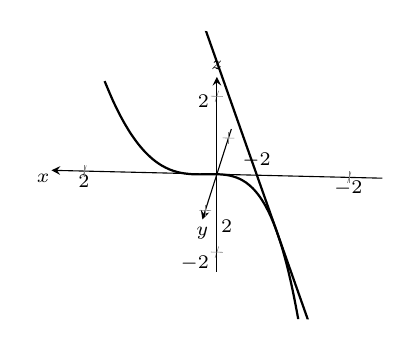
\begin{tikzpicture}[>=stealth]
\begin{axis}%
[width=175pt,tick label style={font=\scriptsize},axis on top,
			axis lines=center,
			view={185}{25},
			name=myplot,
			%xtick={-3,3},minor tick num=2,
			%ytick={-3,3},
			%ztick={-3,3},
			ymin=-2.5,ymax=2.5,
			xmin=-2.5,xmax=2.5,
			zmin=-2.5, zmax=2.5,
			every axis x label/.style={at={(axis cs:\pgfkeysvalueof{/pgfplots/xmax},0,0)},xshift=-3pt,yshift=-3pt},
				xlabel={\scriptsize $x$},
			every axis y label/.style={at={(axis cs:0,\pgfkeysvalueof{/pgfplots/ymax},0)},xshift=0pt,yshift=-5pt},
				ylabel={\scriptsize $y$},
				every axis z label/.style={at={(axis cs:0,0,\pgfkeysvalueof{/pgfplots/zmax})},xshift=0pt,yshift=4pt},
				zlabel={\scriptsize $z$}
			]

\addplot3[domain=-1.5:1.5,,thick,smooth,samples y=0,{\colorone},samples=30,] ({x},{x^2},{x^3});

\addplot3[domain=-1:1.5,,thick,smooth,samples y=0,{\colortwo},samples=30,] ({-1+x},{1-2*x},{-1+3*x});

%\draw[thick,->,{\colortwo}] (axis cs: 0,1,1.57) -- (axis cs: -1,1,2.57) node (A) {};
%\draw[thick,->,{\colortwo}] (axis cs: 0,0,0) -- (axis cs: -1,0,1) node (B) {};


\end{axis}

%\draw (A) node [ above] {\scriptsize $\vec r\,'(\pi/2)$};
%\draw (B) node [shift={(-5pt,5pt)}] {\scriptsize $\vec r\,'(\pi/2)$};



\end{tikzpicture}












